%%%%%%%%%%%%%%%%%%%%%%%%%%%%%%%%%%%%%%%%%%%%%%%%%%%%%%%%%%%%%%%%%%%%%%%%%%%
\fancyChapter{Introduction}[]
\label{chap:intro}
%%%%%%%%%%%%%%%%%%%%%%%%%%%%%%%%%%%%%%%%%%%%%%%%%%%%%%%%%%%%%%%%%%%%%%%%%%%

The beginning of a vision textbook is always predictable: anatomy of the retina first, then onto how rods and cones capture light, contrast, and color.  From there, the chapters progress through orientation, motion, and depth (usually along with some classic visual illusions).  This is baked into the foundation of what visual perception is, and how it is taught to students and future researchers in turn. 

But these foundations follow an implicit pattern: the processing of all the aforementioned scene or object properties center around how visual processing recovers information about what is there in the present, local environment.  Even as the discussion advances to how perception also forms mental representations of relatively complex properties (e.g.~of surfaces, \cite{nakayama_visual_1995}; of objects and object files, \cite{kahneman_reviewing_1992}; see \cite{scholl_objects_2001} for a review), the focus remains on parsing what's immediately present in the visual field.  So when asked about the \textit{purpose} of perception, the most common explanation reflects this precedent --- that ‘seeing’ is for answering some form of the question “\textit{What’s out there?}”.   

In contrast, this dissertation proposes a fundamentally different approach --- that ‘seeing’ is for answering the questions “\textit{What’s happening?}”, “\textit{What just happened?}”, and “\textit{What’s about to happen?}”.  These latter questions possess a crucial aspect that is missing from the classic view of visual perception: the element of time. "What's happening?" implies that an event is currently unfolding, "What just happened?" implies that prior events led to the current state, and "What's about to happen?" implies that future events will soon unfold.  It makes sense that we form static representations of static scenes --- e.g.~when viewing a wooden chair, we can encode its brown color, the shape of its backrest, the spatial location it occupies, etc.  And similarly, it makes sense that we form dynamic representations of dynamic scenes --- e.g.~when viewing that same chair rocking back and forth, we can encode the direction, speed, and frequency of its motion. But this straightforward division overlooks an important dimension.  Because our experience of the world is intrinsically linked to the progression of time, perhaps even when viewing an image where nothing is actually moving (and time is not visibly progressing), the human mind nevertheless remains oriented to temporal processing. In other words, even when some visual input is \textit{static}, perhaps the mind cannot help but recover the \textit{underlying dynamics} of the scene.

In short, this dissertation will present a novel view of how visual perception works using three case studies: (1) intuitive physics, (2) causal history, and (3) environmental affordances and visual routines.  These case studies will illustrate how visual perception is surprisingly rich and sophisticated, as even when processing certain \textit{static} scenes, it extracts properties and forms visual representations that are inherently \textit{dynamic} --- reconstructing not only the deep underlying structure of the scene, but also how the scene \textit{came to be} and how the scene could \textit{continue to unfold}.  In the remainder of this introduction, I will describe why each of these case studies is critical for demonstrating this theme.

%%%%%%%%%%%%%%%%%%%%%%%%%%%%%%%%%%%%%%%%%%%%%%%%%%%%%%%%%%%%%%%%%%%%%%%%%%%
\section{Why Intuitive Physics?}
%%%%%%%%%%%%%%%%%%%%%%%%%%%%%%%%%%%%%%%%%%%%%%%%%%%%%%%%%%%%%%%%%%%%%%%%%%%
Psychologists have long been fascinated by the remarkable sensitivity of the human mind to patterns and regularities.  And surely, of all the regularities in the world, the principles of physics must be the most fundamental and predictable among them.  Gravity will always pull objects down towards the earth’s surface, a heavier object colliding with a lighter object will always cause greater displacement of the latter, and objects in motion will always continue in that motion unless acted upon by an external force, etc.  The reliability of these physical rules has led to a burgeoning field in the study of \textit{intuitive physics}, of how our minds may (or may not) successfully evaluate physical properties in the world around us. 

\begin{figure}
    \centering
    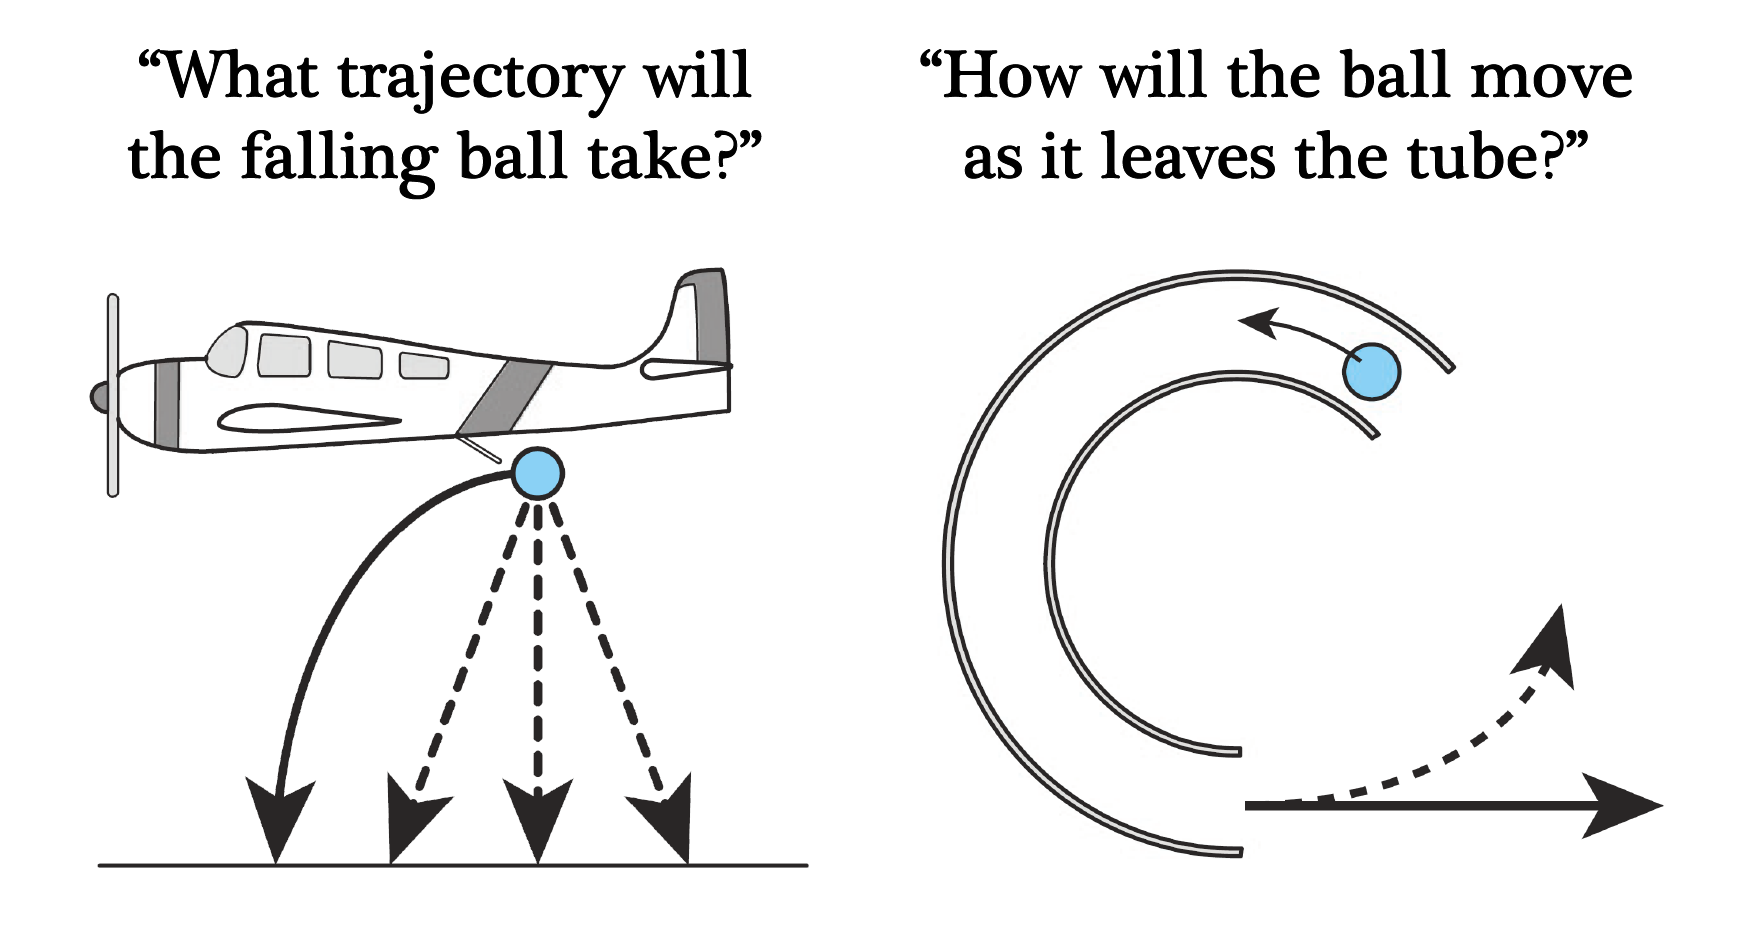
\includegraphics[width=\textwidth]{figures/IntroFig/planefig.pdf}
    \caption
    {\textit{Examples of various intuitive physics task questions}. Solid lines depict the correct answer, while dotted lines depict the frequent mistakes people make. Figure adapted from \cite{kubricht_intuitive_2017}.}
    \label{fig:IntroFig_1}
\end{figure}

The field of intuitive physics is rooted in classic studies such as those depicted in \cref{fig:IntroFig_1}.  For example, when asked to draw the trajectory of a ball rolling out of a curved tube, most people fail to draw the correct (straight) trajectory, and instead incorrectly draw a bent trajectory similar to that of the tube’s curvature \parencite{mccloskey_curvilinear_1980, kaiser_intuitive_1986}.  Or when asked to draw the trajectory of a ball falling from the hand of a person walking (or flying plane, as in \cref{fig:IntroFig_1}), most people fail to draw the correct (parabolic) path that accounts for both vertical and horizontal motion, and instead incorrectly draw the ball falling straight down (e.g.~\cite{mccloskey_alone_1983, mccloskey_etal_1983}).  Other classic studies have also asked participants to judge the relative mass of two colliding objects (e.g.~\cite{gilden_understanding_1989}; \cite{todd_visual_1982}).  These studies share a common theme: (1) that people are error-prone on these tasks, especially when heuristics fail them, and (2) that intuitive physics is centrally a matter of higher-level reasoning and decision-making.  

This perspective has thus been perpetuated into the modern day, as a majority of behavioral tasks in intuitive physics studies still ask participants direct questions about the physics present in a scene, such as “Will the tower fall?” (in precarious-looking towers of varying degrees, e.g.~\cite{battaglia_simulation_2013, hamrick_inferring_2016, mitko_when_2020}), where liquid will flow (e.g.~when encountering obstacles \cite{bates_humans_2015}), how a ball will fall (e.g.~when a pendulum is cut; \cite{smith_different_2018}), which objects have greater mass (e.g.~in two object collisions; \cite{jacobs_learning_2000,jacobs_learning_2001}), and whether some object will get knocked off a table (after being hit by another object; \cite{mitko_dedicated_2024}).  These studies, although all important demonstrations of human cognitive abilities, simply cannot distinguish whether their results are due to people successfully (or unsuccessfully) \textit{thinking} about physics to make predictions, or whether they simply \textit{see} the physics in a scene.

In \Cref{chap:PsychSci2023}, I thus begin by arguing that our appreciation of physical properties --- specifically, of gravity and how it affects object interactions in rigid and soft materials --- occurs \textit{spontaneously}, as part of visual processing itself.  Prior to its publication, other intuitive physics studies (even those that also involved soft materials such as cloth) either used overt judgment tasks (such as directly asking participants to identify different types of cloth folds; \cite{phillips_veiled_2020}) or employed tasks where intuitive physics would have benefited performance; \parencite{little_whats_2020}.  \Cref{chap:PsychSci2023} was thus, to my knowledge, the first empirical demonstration of spontaneous perception of intuitive physics even though it was neither relevant to the task at hand, nor beneficial for task performance. 

\Cref{chap:PsychSci2023} then explores how intuitive physics offers a unique perspective into the idea of \textit{dynamicism} in perception.   It is, of course, natural to watch some animation of colliding balls, and represent the dynamics that are actively playing out in front of you --- e.g.~the speeds at which the balls collide, where the balls start positions were, where the balls roll, the relative masses, etc.  In contrast, consider the following incredibly understudied (yet incredibly rich) visual stimulus: a single, static image of an object completely covered by a cloth  that is draped over it.  Here, the visual representation would intuitively include static information, such as the color of the cloth, texture of the material, and the bends or folds in the cloth's surface.  But I propose that even in this static image, we form dynamic visual representations based on the intuitive physics underlying the scene.  In this particular example, we may not only represent the dynamics of how the soft material of the cloth (e.g.~mass, stiffness) physically interact with those of the solid object beneath the cloth (with its own mass and rigid structure), but also with gravity (which is the cause of particular cloth folds, how it bends over the edges of the object underneath, etc). Such representations would be critical for perception, because it would enable the agent to act upon the scene in various ways: grasping the object at appropriate structural points rather than loose cloth areas, accounting for the cloth shifting when the structure is moved, etc.

I thus propose that the dynamic reconstruction of the physics in this scene type enable us to distinguish cloth folds that are merely \textit{superficial} (highly variable, theoretically would vary with each re-draping of the cloth), vs.~folds that are indicative of the \textit{deep underlying structure} (i.e. of the hidden object underneath).  I will demonstrate these ideas empirically: across change detection and probe comparison tasks in static cloth-covered object images --- neither of which require any intuitive physics to complete --- observers nevertheless spontaneously (a) perceive intuitive physics of gravity, soft materials, and rigid objects, and (b) \textit{prioritize} features that reflect the structure of the object beneath the cloth. In short, \Cref{chap:PsychSci2023} illustrates how visual processing is not simply about answering “What’s out there?”, but rather, “What’s happening?”


%%%%%%%%%%%%%%%%%%%%%%%%%%%%%%%%%%%%%%%%%%%%%%%%%%%%%%%%%%%%%%%%%%%%%%%%%%%
\section{Why Causal History?}
%%%%%%%%%%%%%%%%%%%%%%%%%%%%%%%%%%%%%%%%%%%%%%%%%%%%%%%%%%%%%%%%%%%%%%%%%%%
\begin{figure}
    \centering
    \includegraphics[width=\textwidth]{figures/IntroFig/causalhist_upscaled.pdf}
    \caption
    {\textit{Examples of different objects with different causal history}. Figure adapted from \cite{chen_perception_2016}.}
    \label{fig:IntroFig_2}
\end{figure}

It has been said that “the shape of an object often seems to tell us something about the object's history” (\cite{leyton_inferring_1989}, p.~1), and indeed, this quote seems to ring true upon visually assessing any of the items in \cref{fig:IntroFig_2}.  When we look at the bitten cookie, we can identify the particular jagged edge that interrupts its otherwise circular form.  But section is not merely an "absence" --- instead, we perceive this as a "missing" piece, one that suggests a particular transformation: \textit{getting bitten}.  And simultaneously, as part of this processing, we extract that it once had a whole, complete form (prior to getting bitten). Similarly, when viewing the aluminum can with its collapsed sides, we do not just see a complex shape with irregular contours --- instead, we perceive this as (a) having an original, unperturbed state where it was once a smooth cylindrical structure, and (b) the current form being the result of \textit{getting crushed}.

These examples raise the possibility that the visual processing of these static images entails dynamic representations of a scene's \textit{causal history}:  not only the current, transformed state of the object (the bitten cookie, the crushed can, the twisted towel), but also (a) an implicit representation of its original, untransformed state (the whole cookie, the intact can, the flat towel), and (b) the type of causal transformation it was subjected to (biting, crushing, twisting).  

There exists surprisingly little empirical work on this provocative notion of causal history. When shown various novel 3D objects \parencite{fleming_getting_2019, schmidt_visual_2019}, or familiar real world materials \parencite{schmidt_identifying_2018}  that were subjected to different transformations such as "twisting", "bending", "inflating/bloating", or "hammering", participants were indeed able to successfully group and categorize objects that had undergone identical causal history transformations. Additionally, participants judged the symmetry axes of irregular "bitten" shapes to be more similar to their pre-transformation "whole" counterparts than to "smoothed" shapes that shared the same concavities but lacked causal history \parencite{sprote_visual_2016}. Although it is certainly important to understand that the human mind is able to judge, categorize, and assess causal history, these studies cannot truly distinguish whether their results are due to people successfully (or unsuccessfully) \textit{thinking} about causal history, or whether they simply \textit{see} how the scene came to be.

In perhaps the only empirical exploration of the perception of causal history, Chen \& Scholl (\citeyear{chen_perception_2016}) showed observers brief animations of squares undergoing two different transformations: either “intrusions” (as when a square-shaped clay is indented with a finger) or “impositions” (as when a piece of a square-shaped clay is cut out by a cookie-cutter). Despite the animation consisting of just two frames (first frame: whole square; second frame: intruded or imposed square), observers experienced illusory apparent motion more frequently with the intruded square than the imposed square. This difference was attributed to causal history, since imposition transformations (i.e. when clay is cut by a cookie-cutter) must occur instantaneously, whereas intrusion transformations (i.e. when clay is indented by a finger) can occur gradually, as the material is pressed further inwards.\footnotemark

\footnotetext{There exists actually one other empirical paper using a perception-based task to investigate causal history (using visual search; \cite{brenner_searching_2020}). However, their results are mixed, and they therefore do not argue for the perception of causal history in the same way that Chen \& Scholl (\citeyear{chen_perception_2016}) do.}

In \Cref{chap:casual_hist}, I argue that causal history is far more prominent than ever previously considered. Actually, this was a possibility inadvertently raised by \Cref{chap:PsychSci2023} (exploring intuitive physics), that goes beyond the original point of dynamic representations of physical forces present in certain static scenes --- specifically, a possibility that concerns reconstructing the progression of \textit{time}. When viewing a cloth-covered object and recovering the object beneath the cloth, visual processing essentially retraces \textit{how the scene came to be} in the first place.  After all, according the rules of physics, there is a set order of operations for how this kind of scene was constructed: the rigid object \textit{must} have been placed first, and the cloth was draped over it afterwards.  This idea can then easily be extended to other types of scenes.  When viewing a simple stack of books, for example, the underlying intuitive physics necessitate a specific causal history: that the stack must have been built from bottom to top, due to gravity. 

\Cref{chap:casual_hist} thus argues that even when showing observers static scenes (such as two blocks vertically stacked), we spontaneously form dynamic representations of causal history --- based on the underlying intuitive physics. In particular, \Cref{chap:casual_hist} demonstrates that intuitive physics-based causal history is so robust that it can even sometimes override sensory input: two blocks (stacked on top of each other) that appear simultaneously are often misperceived as having appeared sequentially (specifically, bottom-to-top, in line with the causal history), and two blocks (stacked on top of each other) that appear sequentially from top-to-bottom are often misperceived as having appeared simultaneously (as if the causal history canceled out the true sensory input).  In short, \Cref{chap:casual_hist} illustrates how visual processing is not simply about answering “What’s out there?”, but rather, “What just \textit{happened}?”


%%%%%%%%%%%%%%%%%%%%%%%%%%%%%%%%%%%%%%%%%%%%%%%%%%%%%%%%%%%%%%%%%%%%%%%%%%%
\section{Why Affordances and Visual Routines?}\label{sec:why_visual_routines}
%%%%%%%%%%%%%%%%%%%%%%%%%%%%%%%%%%%%%%%%%%%%%%%%%%%%%%%%%%%%%%%%%%%%%%%%%%%
It’s easy to take seeing for granted when considering our mental lives, perhaps because it seems so very fast and reflexive.  In particular, many properties seem to be extracted during visual processing in a way that seems both (phenomenologically) instantaneous and to occur without a specific intention.   This is evident in our old, reliable example of perceiving color.  When you view an object, you seem to perceive its color without any appreciable delay, and without having to make a deliberate effort to see that color.  Likewise for the perception of a line’s orientation, an animal’s size, or a car’s direction of motion.  And this even seems to hold for the perception of stimuli that we know are extracted over multiple discrete steps in a way that involves some ‘unconscious inference’ unfolding over hundreds of milliseconds — such as the perception of amodally completed surfaces (e.g.~\cite{rauschenberger_masking_2001}).  (Indeed, such displays are infamous precisely because the resulting surfaces seem to be perceived instantly and automatically.)

\begin{figure}
    \centering
    \includegraphics[width=\textwidth]{figures/IntroFig/coloring.pdf}
    \caption
    [\textit{Overlapping colorful outlines and shapes scattered around.} See text in \Cref{sec:why_visual_routines} for details]
    {\textit{See text in \Cref{sec:why_visual_routines} for details}.}
    \label{fig:IntroFig_3}
\end{figure}

There are, however, fascinating exceptions to this rule.  For example, take a moment to glance at \cref{fig:IntroFig_3} before reading on. ... Now consider some questions that could be asked about that figure.  What colors were present?  What shapes were present?  You can probably answer these questions immediately, from memory — indicating that this property was extracted even before you were asked the question, just as a part of natural viewing (even if your memory isn’t necessarily perfect).  But what about this question: Does the black disc lie inside or outside the purple outline?  You probably don’t know the answer yet, which indicates that this property was not extracted involuntarily during natural viewing.  When you look back at \cref{fig:IntroFig_3}, of course, you can answer this question too --- and you can do so merely by looking.  But notice that even here you can’t answer the question immediately: whereas you see color seemingly instantaneously, seeing which boundaries encompass which shapes is appreciably deliberate, dynamic, and temporally extended (as you must trace the purple outline of interest, mentally ‘color in’ that outline, and track which shapes fall inside it).  This type of visual operation that underlies your ability to answer the is-it-inside-or-outside question has been coined as a type of \textit{visual routine} \parencite{selst_visual_1995, ullman_visual_1984, ullman_chapter_1996}, along with other visual operations that concern relative spatial relations (e.g.~whether two objects lie along the same contour, or whether one particular object is to the right or left of another particular object). Since its proposal, visual routines have also been hypothesized to support other important visual operations such as grouping \parencite{watt_function_2000} and figure-ground processing \parencite{poort_role_2012}.

Visual routines are therefore ideal for exploring how even static visual scenes (including relatively complex ones like \cref{fig:IntroFig_3}) involve \textit{dynamic operations}.  But visual routines hold a particular place within visual processing.  Because just as the dynamicism of visual routine operation is a part of its phenomenology, so too is its task-dependency.  Look back at \cref{fig:IntroFig_3}.  One reason for thinking that visual routines must exist as a separate sort of operation in visual processing is just that it would often not be possible for them to operate incidentally (without a specific goal or task), for reasons of brute computational explosion.  Our example contained 6 shapes and 3 colored outlines, and already it would not be feasible, even in principle, to “pre-compute” such answers prior to the question being posed, simply because there would be too many X/Y pairs of shapes and outlines to consider the relative relations for.  In the real world of uncontrolled, complex visual environments crowded with even greater numbers of objects than in \cref{fig:IntroFig_3}, it would be even less computationally feasible to assess all relations at once.  Indeed, this need to be invoked ‘on demand’ can be seen in how visual routines are defined in the literature, for example, “[t]he appropriate routine to be applied in a given situation depends on the goal of the computation” (\cite{ullman_visual_1984}, p.~153), and such routines are engaged only “in certain visual tasks” (\cite{jolicoeur_curve_1986}, p.~137). 

\begin{figure}
    \centering
    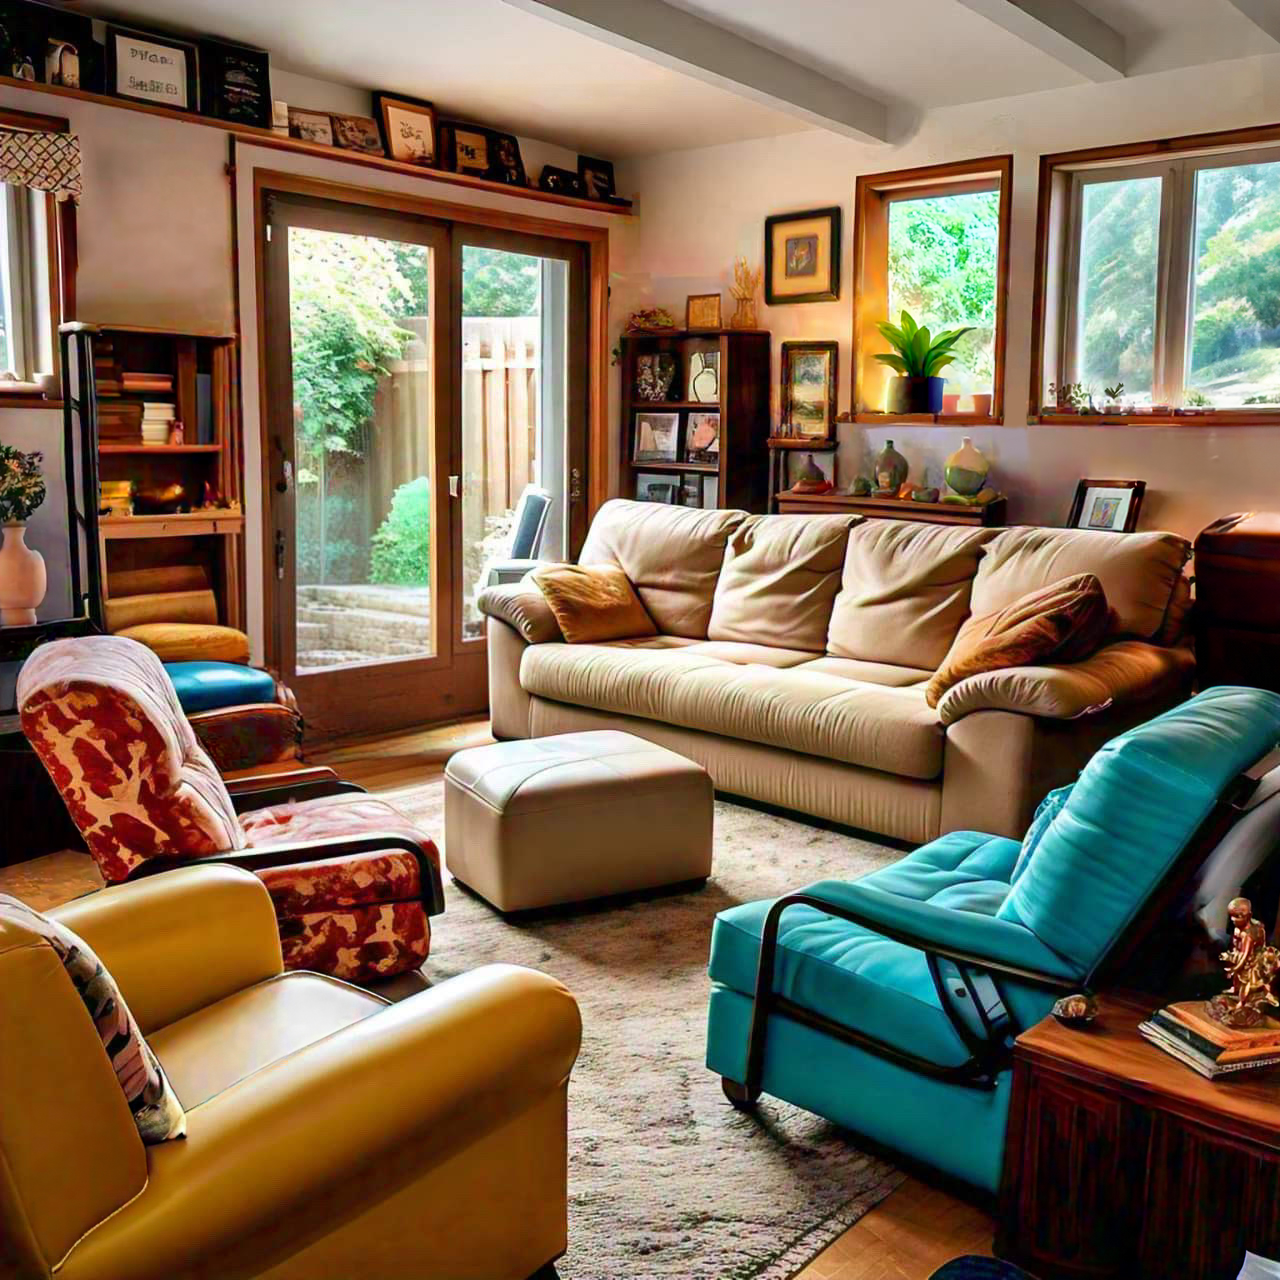
\includegraphics[width=\textwidth]{figures/IntroFig/clutteredroom.jpg}
    \caption
    {\textit{A cluttered room}. There are ‘navigable’ paths to take within it.}
    \label{fig:IntroFig_4}
\end{figure}

\Cref{chap:JEPG2024} will begin by arguing that visual routines can indeed be spontaneous, in certain scenes, as enabled by '\textit{affordances}' (à la James Gibson, \citeyear{gibson_ecological_1979}). What are affordances? Take a look at \cref{fig:IntroFig_4}. ...  Even though the space contains numerous pieces of furniture and objects, we seem to be able to immediately discern certain pathways through this cluttered room.  This sensitivity to the the open spaces --- pathways that we are able to locomote and navigate through --- exemplify a specific type of affordance: \textit{navigational affordances} (for a review, see \cite{gregorians_affordances_2022}).  Previous work has investigated navigational affordances especially in neural contexts. In particular, the Occipital Place Area (OPA) corresponds with coding for potential paths or routes through a scene \parencite{bonner_coding_2017, bonner_computational_2018}, and electrophysiological evidence supports early processing of the number of possible paths or exits \parencite{harel_early_2022}.  Furthermore, recent behavioral evidence shows that paths leading to doors (exits) are extracted even when task-irrelevant \parencite{belledonne_automatic_2021, belledonne_navigational_2022}.

\Cref{chap:JEPG2024} thus applies this concept of navigational affordances to static images of \textit{mazes}. While mazes can certainly be traditionally solved by tracing paths with a pencil or finger, they can also be solved without any physical tools: by \textit{mentally} tracing through the paths.  I demonstrate that this 'mental path tracing' is spontaneous, occurring regardless of task demand --- due to certain scenes' navigational affordances invoking the visual routine of 'curve tracing'.  Specifically, when observers are tasked with comparing the [aesthetic appearance] of two probes present within the paths of the maze --- a task that has nothing to do with visual routines nor affordances --- observers nevertheless take longer to respond depending on the the probes' \textit{pathwise} distance from each other, and not their brute Euclidean distance.

\Cref{chap:JEPG2024} will then leverage visual routines and affordances as a powerful lens through which to explore dynamism in perception --- in how they enable dynamic representations of the feasible \textit{future}. I propose that when we perceive a scene containing paths and obstacles, we don't merely register the static arrangement of elements --- we spontaneously extract information about potential movement through the scene. This involves reconstructing the navigability of spaces (as in \cref{fig:IntroFig_4}) and traversable future paths (such as how to get from one probe to another). Even when viewing completely static displays, our visual system appears to spontaneously track possible future trajectories through the environment, accounting for likely future actions. In this way, \Cref{chap:JEPG2024} illustrates how visual processing is not simply about answering “What’s out there?”, but rather, “What’s \textit{about to} happen?”


%%%%%%%%%%%%%%%%%%%%%%%%%%%%%%%%%%%%%%%%%%%%%%%%%%%%%%%%%%%%%%%%%%%%%%%%%%%
\section{Overview of the Current Chapters}
%%%%%%%%%%%%%%%%%%%%%%%%%%%%%%%%%%%%%%%%%%%%%%%%%%%%%%%%%%%%%%%%%%%%%%%%%%%

Across the studies in this dissertation, I suggest that perception is about \textit{seeing what matters} --- be it the deep, underlying structure of the scene (\Cref{chap:PsychSci2023}), the probable past (\Cref{chap:casual_hist}), or the feasible future  (\Cref{chap:JEPG2024}).  I discuss this in the context of intuitive physics, of causal history, and of affordances and visual routines respectively.  Each of the chapters will highlight different aspects the critical theme: even when viewing certain static scenes, visual representations are inherently dynamic.  \Cref{chap:PsychSci2023} will begin with the representation of intuitive physics underlying images of cloth-covered objects, \Cref{chap:casual_hist} will capture the representation of causal history underlying images of stacked blocks, and \Cref{chap:JEPG2024} will explore the representation of navigational affordances underlying images of mazes and obstacle-filled scenes.

These chapters were written as individual journal articles, and they are all either published \parencite{wong_seeing_2023, wong_spontaneous_2024}, or in preparation for submission.  As a result, they stand on their own, and can be read independently, in any order. 

